\section{RESULTS AND DISCUSSION}


\begin{table}[h]
\caption{Numerical results}
\label{table:results}
\begin{center}
\begin{tabular}{c||cc|cccc}
\hline
Method & \multicolumn{2}{c|}{Similarity (\%)} & \multicolumn{4}{c}{\gls*{fji} (\%)} \\
\hline
 & B0 & \glspl*{dwi} & Av. & \gls*{csf} & \gls*{wm} & \gls*{gm} \\
\hline
\gls*{fmb} & $80.05$ & $96.26\pm.06$ & $93.00$ & $88.57$ & $96.74$ & $94.02$ \\
\hline
\gls*{reb} & $91.00$ & $97.65\pm.03$ & $96.64$ & $94.31$ & $98.26$ & $96.75$ \\
\hline
\gls*{t2b} & $64.58$ & $90.10\pm.13$ & $79.19$ & $66.31$ & $89.85$ & $82.14$ \\
\hline
\end{tabular}
\end{center}
\end{table}

\begin{figure*}[tpb]
   \centering
   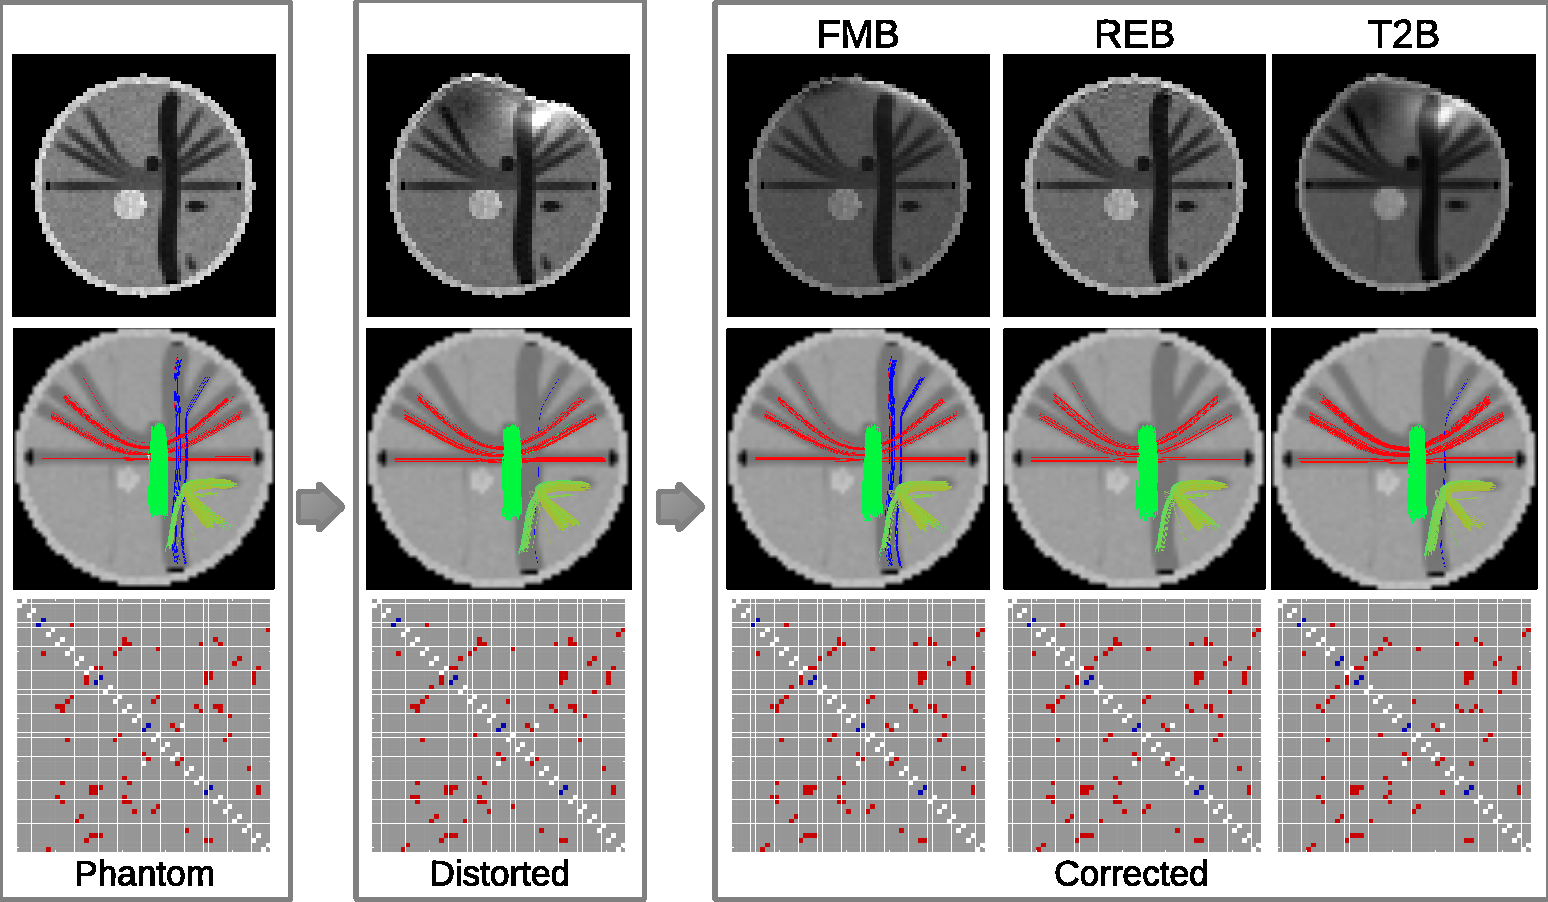
\includegraphics[width=0.9\textwidth]{Fig02-Results}
   \caption{The three major stages of the evaluation framework,
   along with the associated visual results. First row represents
   a sagittal section of the B0 volume. In second row, the outcome
   of tractography, showing only tracks that connect two different
   network nodes. Third row shows the connectivity matrix associated
   to the corresponding tractography in second row. The }
   \label{fig:results}
\end{figure*}

The results of the proposed experiments are summarized
in \autoref{fig:results} and \autoref{table:results}.
The remaining of this section provides extended descriptions
and interpretation of results.

\subsection{Geometrical correctness}

The three methods under study achieved good results in
terms of geometrical accuracy, as it is shown in the first
row of \autoref{fig:results}. The best numerical scores
were obtained with the \gls*{reb} method (\autoref{table:results}),
that achieved a weighted average overlap of $96.64\%$. Second
best were obtained with \gls*{fmb}. Geometrical correctness
is fundamental in connectivity analysis to spatially locate the
\glspl*{roi} that will define the nodes of the final connectivity
matrix. The clear difference of accuracy between \gls*{reb} and \gls*{fmb}
with respect the \gls*{t2b} might point out that the latter is
not an appropriate method for susceptibility correction.	


\subsection{Signal loss recovery}

A second workflow evaluated the different correction 
methodologies to show the similarity of the recovered
signal with respect the original (undistorted) one. 
In this second study, \gls*{reb} performed significantly
better than the other two methods, as reported
in \autoref{table:results}. \gls*{reb} scored a $91.0\%$
similarity index for the B0 volume and an average $97.65\%$
for the remaining 31 \glspl*{dwi}. Again, the second
qualified was \gls*{fmb}, which achieved very close results
for the \glspl*{dwi} ($96.26\%$) but not as good for the B0
volume. Visual inspection of the recovered data confirm the 
results presented in the Table (\autoref{fig:results}, first
row). Finally, \gls*{t2b} confirmed that its correction
can not be compared, even with using intensity correction with
the determinant of the deformation field.

\subsection{Impact on tractography and connectivity}

The final objective of the present work was to characterize
in a reproducible manner the effects of susceptibility distortions
on the connectivity analysis. The gold-standard connectivity
matrix contained a total of 1888 tracks, with an average
length of $40.88\pm8.06$mm. After distortion, this numbers
changed to a total of 1855 tracks and a characteristic length
of $40.64\pm8.12$mm. Therefore, very specific tracks were affected
by distortion, as it was intended on the experiment. These differences
are highlighted in the second row of \autoref{fig:results}. Two
main effects can be expected from susceptibility distortion,
depending on the intensity of the deformation. Those areas exposed
to a slight deformation showed an increase of variability when
the signal is not orthogonal to the phase encoding axis 
(\autoref{fig:results}, second row, A) or an
increase of directional anisotropy of diffusion
(\autoref{fig:results}, second row, B), when the
diffusivity is orthogonal to the distortion.
Finally, regions subjected to severe susceptibility-induced 
distortion, some tracks were lost (\autoref{fig:results},
second row, C).

After \gls*{fmb} correction, a total of 1905 tracks 
of $40.53\pm8.07$mm. were obtained (\gls*{frr}=$100.9\%$). 
For \gls*{reb} these figures are 2283 tracks (\gls*{frr}=$120.93\%$) 
and $41.15\pm7.60$mm. 
length. Finally, \gls*{t2b} yielded 2495 (\gls*{frr}=$132.1\%$) tracks and 
$40.60\pm7.81$mm. Although these results pointed at
\gls*{fmb} as the best method, the visual inspection
of tractography suggested that again, only \gls*{reb}
was successful recovering lost connections and reducing
variability of tracks over impacted regions. 

\subsection{Discussion}

Even though all the surveyed methods produced visually sound results,
our study suggested that \gls*{reb} is the most accurate
methodology for susceptibility-induced distortions in
\gls*{epi}. Nonetheless, \gls*{fmb} achieved very accurate
scores, with better results on tractography as compared to
\gls*{reb}. Clearly, the \gls*{t2b} method did not achieve
the necessary high-standards to recommend its use.
We recall that this last conclusion is potentially biased 
by the gold-standard generation
methodology, as it also used \gls*{fmb}.
A second limitation of this work is that \gls*{psf}-based methods 
could not be included on comparisons for two reasons.
First, the necessary \gls*{psf} map consistent with the synthetic
phase-difference map was not available. Second, to our knowledge,
there are no \gls*{psf}-based methods with readily available 
implementations we could have used for comparisons. 
In practice, this second limitation is not relevant because
typical acquisition protocols usually include one or more
datasets among field mapping, reversed-encoding B0 or \gls*{t2},
but they do not include the necessary \gls*{psf} mapping.

Therefore, this work reviewed the most common
correction methodologies using a new evaluation
framework, and reporting the benchmark results.